\chapter{Presenting a talk}
\label{app:Talk}

When presenting your thesis work in a talk, you will want to convey
an overview of your thesis as a whole. However, you must pick and
choose what to emphasize since time will be limited. There is no
formal oral defense requirement for the senior thesis (although
there is for an Honor's Thesis). However, the department encourages
students to make at least one formal presentation on their research.
All students doing a senior thesis, and especially those receiving
department funding, are expected to participate in the annual Spring
Research Conference held each March in the College of Physical and
Mathematical Sciences at BYU. Depending on available travel
resources, students may also have the opportunity to present a talk
at a professional meeting outside of campus.

For short talks, you should have no more than two thirds as many
slides as you have minutes allocated for your talk. For longer
talks, you should have somewhat fewer slides. Create a title page
which acknowledges everyone who has contributed to the work. Prepare
an outline slide that will let the audience know what you are going
to be presenting. (If time is extremely short (e.g. 7 minute talk),
you may dispense with the outline slide.) At least a third of your
talk should be introductory in nature, providing background that
will help the audience appreciate the work. The main goal in giving
a talk is to convey to the audience a sense that your work is
important; the goal is not to give the audience a lot of details
which they will never remember nor even get straight in the first
place. Less is more. A conclusion slide can be used to remind the
audience of your main points and to summarize the significance of
your work. Keep it brief. The conclusion slide may be omitted if it
seems too redundant, depending on how you presented the
material[10].

\begin{figure}
    \centerline{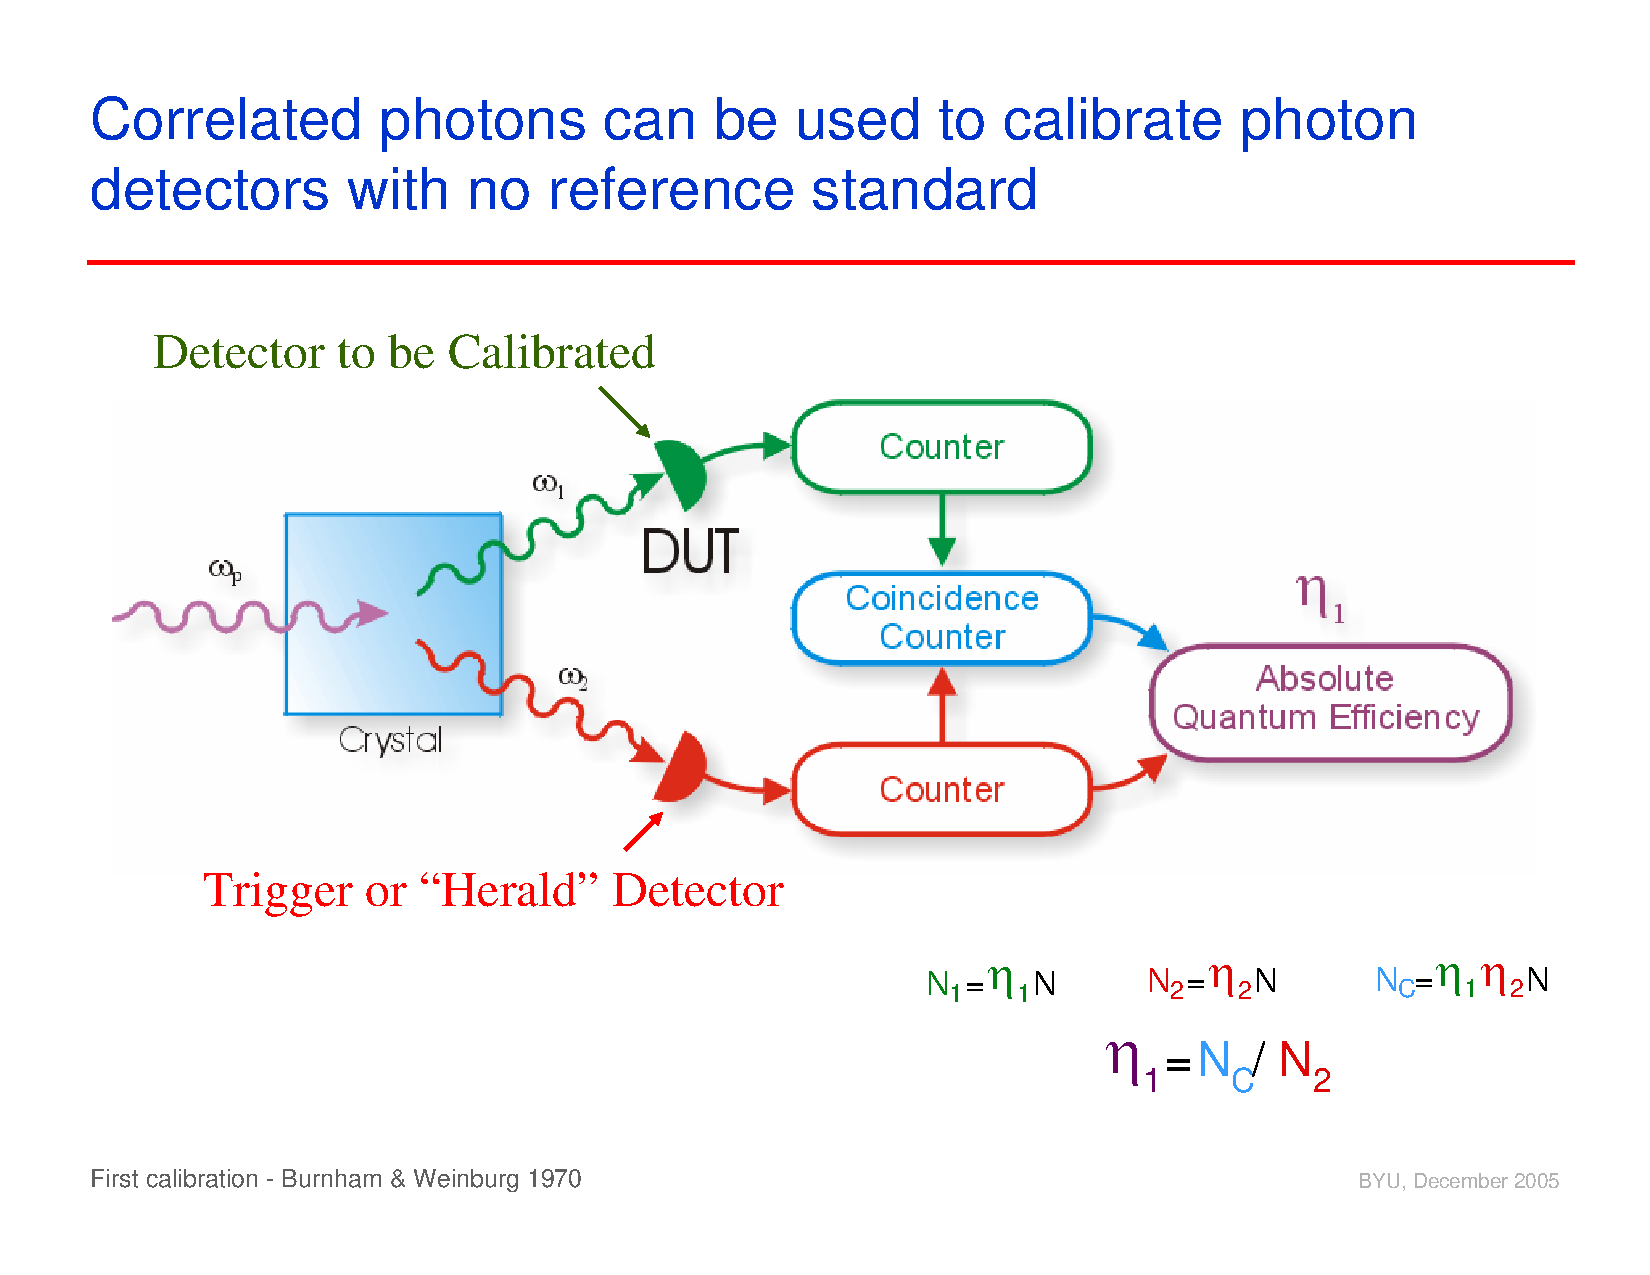
\includegraphics[width=6.5in]{Slide}}
    \caption{\label{fig:Slide} A sample slide from a presentation}
\end{figure}

Many of the figures that you prepare for your thesis will be useful
for your slide presentation. Keep slides simple and uncluttered.
Include less information on a view graph than you plan to talk
about. Be sure that important labels are present (such as the units
on graph axes). Use large fonts so that your slides are easy to
read, even for people in the back. It is a good idea to place a
single large ``header" sentence at the top of each view graph (no
more than two lines using a 24 point font). Think of the main idea
that you want an audience member to get from a slide, and use that
for the header sentence. Use color freely, but keep it tasteful.
Figure~\ref{fig:Slide} shows an example of a view graph.

Practice your talk to yourself and to others in your research group,
especially your advisor. Time your practice runs. If you do not
practice, you will most likely give too many extraneous details and
muddle through or even miss your main points for lack of time, a
sure recipe for a boring talk.
